% The first command in your LaTeX source must be the \documentclass command.

\documentclass[sigconf]{acmart}
 % Do not change for SPAA'19

\settopmatter{printacmref=true}
  % mandatory for SPAA'19

\fancyhead{}
  % do not delete this code.

\usepackage{balance}
  % for creating a balanced last page (usually last page with references)

% defining the \BibTeX command - from Oren Patashnik's original BibTeX documentation.
\def\BibTeX{{\rm B\kern-.05em{\sc i\kern-.025em b}\kern-.08emT\kern-.1667em\lower.7ex\hbox{E}\kern-.125emX}}
    
% Rights management information. 
% This information is sent to you when you complete the rights form.
% These commands have SAMPLE values in them; it is your responsibility as an author to replace
% the commands and values with those provided to you when you complete the rights form.
%
% These commands are for a PROCEEDINGS abstract or paper.

\copyrightyear{2019} 
\acmYear{2019} 
\setcopyright{acmcopyright}
\acmConference[UMAP'19 Adjunct]{27th Conference on User Modeling, Adaptation and Personalization Adjunct}{June 9--12, 2019}{Larnaca, Cyprus}
\acmBooktitle{27th Conference on User Modeling, Adaptation and Personalization Adjunct (UMAP'19 Adjunct), June 9--12, 2019, Larnaca, Cyprus}
\acmPrice{15.00}
\acmDOI{10.1145/3314183.3326364}
\acmISBN{978-1-4503-6711-0/19/06}


% Submission ID. 
% Use this when submitting an article to a sponsored event. You'll receive a unique submission ID from the organizers
% of the event, and this ID should be used as the parameter to this command.
%\acmSubmissionID{123-A56-BU3}


% end of the preamble, start of the body of the document source.

\begin{document}


% The "title" command has an optional parameter, allowing the author to define a "short title" to be used in page headers.
\title{Security And Privacy Of Medical Data}
\subtitle{Challenges For Next-Generation Patient-Centric Healthcare Systems}



% The "author" command and its associated commands are used to define the authors and their affiliations.
% Of note is the shared affiliation of the first two authors, and the "authornote" and "authornotemark" commands
% used to denote shared contribution to the research.
\author{Vladimir Janjic}
\email{vj32@st-andrews.ac.uk}
%\orcid{1234-5678-9012}
\author{Juliana Bowles}
%\authornotemark[1]
\email{jkfb@st-andrews.ac.uk}
\affiliation{%
  \institution{School of Computer Science, University of St Andrews}
  %\streetaddress{P.O. Box 1212}
  %\city{Dublin}
  %\state{Ohio}
  %\postcode{43017-6221}
  \country{United Kingdom}
}

\author{Marios Belk}
\email{belk@cs.ucy.ac.cy}
\author{Andreas Pitsilides}
\email{andreas.pitsillides@ucy.ac.cy}
\affiliation{%
  \institution{University of Cyprus}
  \country{Cyprus}}

% By default, the full list of authors will be used in the page headers. Often, this list is too long, and will overlap
% other information printed in the page headers. This command allows the author to define a more concise list
% of authors' names for this purpose.
\renewcommand{\shortauthors}{Janjic, Bowles, Belk and Pitsilides}

%
% The abstract is a short summary of the work to be presented in the article.
\begin{abstract}
In order to achieve the highest quality of healthcare provision, it is increasingly important to collect highly confidential and personal medical data that has been obtained from a variety of sources, including personal medical devices and to share this through a variety of means, including public networks and other systems whose security cannot be implicitly trusted. Consequently, the future medical centres will be \emph{highly decentralised}, with the data about a single patient residing on a number of different devices, some of which will be completely outside of the medical organisation. This raises a number of issues related to preserving security, privacy and ownerwship of the patient data, while still ensuring that the patients get the best possible medical treatment. The goal of the recently-started \emph{Serums} EU H2020 project is to develop novel mechanisms for collecting, storage, communication and analysis of the medical data, together with novel authentication and authorisation mechanisms, that will enable putting patients in the centre of the future healthcare provision, enhance their personal care, maximise the quality of treatment they receive all the while ensuring trust in the security and privacy of their confidential medical data. 
\end{abstract}


%% ToDo: Fix this!
%
% The code below is generated by the tool at http://dl.acm.org/ccs.cfm.
% Please copy and paste the code instead of the example below.
%
%%%%%%%%%%%%%%%%%%%%%%%%%%%%%%%%%%%%%%%%%%%%%%%%%%%%%%%%%%%%%%%%%%%%%%%%%%%%%%%%%%%
%% \begin{CCSXML}                                                                %%
%% <ccs2012>                                                                     %%
%%  <concept>                                                                    %%
%%   <concept_id>10010520.10010553.10010562</concept_id>                         %%
%%   <concept_desc>Computer systems organization~Embedded systems</concept_desc> %%
%%   <concept_significance>500</concept_significance>                            %%
%%  </concept>                                                                   %%
%%  <concept>                                                                    %%
%%   <concept_id>10010520.10010575.10010755</concept_id>                         %%
%%   <concept_desc>Computer systems organization~Redundancy</concept_desc>       %%
%%   <concept_significance>300</concept_significance>                            %%
%%  </concept>                                                                   %%
%%  <concept>                                                                    %%
%%   <concept_id>10010520.10010553.10010554</concept_id>                         %%
%%   <concept_desc>Computer systems organization~Robotics</concept_desc>         %%
%%   <concept_significance>100</concept_significance>                            %%
%%  </concept>                                                                   %%
%%  <concept>                                                                    %%
%%   <concept_id>10003033.10003083.10003095</concept_id>                         %%
%%   <concept_desc>Networks~Network reliability</concept_desc>                   %%
%%   <concept_significance>100</concept_significance>                            %%
%%  </concept>                                                                   %%
%% </ccs2012>                                                                    %%
%% \end{CCSXML}                                                                  %%
%%%%%%%%%%%%%%%%%%%%%%%%%%%%%%%%%%%%%%%%%%%%%%%%%%%%%%%%%%%%%%%%%%%%%%%%%%%%%%%%%%%

%\ccsdesc[500]{Computer systems organization~Embedded systems}
%\ccsdesc[300]{Computer systems organization~Redundancy}
%\ccsdesc{Computer systems organization~Robotics}
%\ccsdesc[100]{Networks~Network reliability}

%
% Keywords. The author(s) should pick words that accurately describe the work being
% presented. Separate the keywords with commas.
\keywords{datasets, neural networks, gaze detection, text tagging}

%
% A "teaser" image appears between the author and affiliation information and the body 
% of the document, and typically spans the page. 
%\begin{teaserfigure}
%  \includegraphics[width=\textwidth]{sampleteaser}
%  \caption{Seattle Mariners at Spring Training, 2010.}
%  \Description{Enjoying the baseball game from the third-base seats. Ichiro Suzuki preparing to bat.}
%  \label{fig:teaser}
%\end{teaserfigure}

%
% This command processes the author and affiliation and title information and builds
% the first part of the formatted document.
\maketitle

\section{Introduction}

\noindent
In order to achieve the highest quality of healthcare provision, it is increasingly important to collect highly confidential and personal medical data that has been obtained from a variety of sources, including personal medical devices and to share this through a variety of means. Integrating home-based healthcare into a holistic treatment plan is more cost effective, reduces travel-associated risks and costs and increases the quality of healthcare provision. Consequently, the medical centres of the future will be \emph{highly decentralised}, with the data about a single patient residing on a number of different devices, some of which will be reside outside of the trusted networks of the medical organisation. In some cases, cooperation between different health institutions that may reside in different countries, might be required to ensure the patients get the best possible treatment. All this raises a number of issues related to preserving security and privacy of the patient data, together with complying to a combination of different national and international legislations (such as GDPR) that regulate ownership and sharing of that data.

The goal of the recently-started \emph{Serums: Securing Medical Data in Smart Patient-Centric Healthcare Systems} EU H2020 project is to develop novel mechanisms for safe and secure collection, storage, communication and analysis of the medical data. We aim to put patients in the centre of the future healthcare provision, enhance their personal care, maximise the quality of treatment they will receive while ensuring trust in the security and privacy of their confidential medical data. Figure~\ref{fig:smartcentre} shows the example of data sharing in the future-generation smart healthcare centres, where different entities (different classes of users, different parts of the healthcare center system) need to exchange data. The main objectives of the \emph{Serums} project are 

\begin{figure}
  \centering
  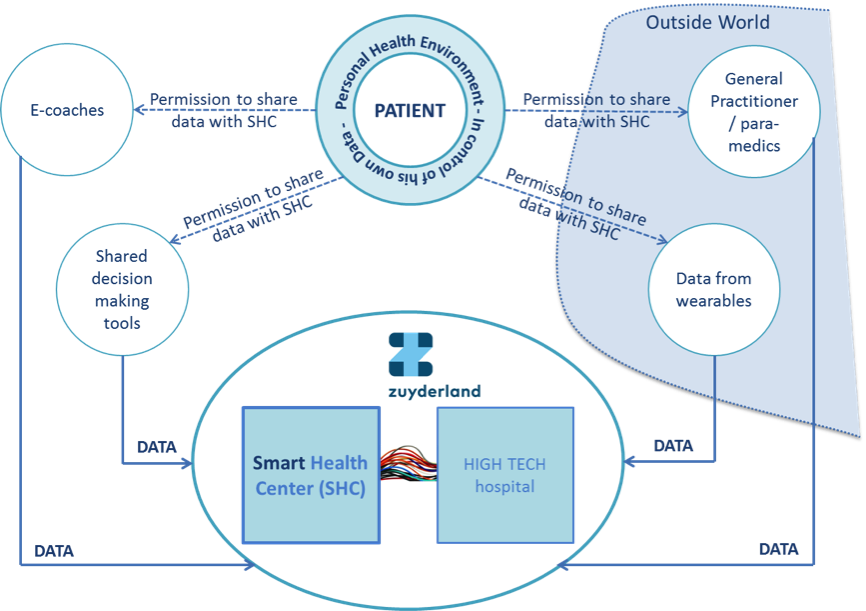
\includegraphics[width=\columnwidth]{SmartHealthCentre.png}
  \caption{Example of Data Sharing in Smart Health Center}
  \label{fig:smartcentre}
\end{figure}
    
\begin{itemize}
\item to develop new techniques that will ensure the \emph{security and protection of personal medical data} that is shared between patients, hospitals and medical practitioners in smart healthcare systems;
\item to integrate personal medical data from multiple sources (e.g.~personal monitoring devices, hospital diagnostics systems, specialists and general practicioners) into a single coherent \emph{smart patient record};
\item to develop \emph{new data analytic techniques} that will be able to take advantage of advances in the availability of heterogeneous real-time personal healthcare information, as part of a holistic smart healthcare system, while respecting privacy and security concerns;
\item to develop/enhance \emph{authentication and trust mechanisms} that ensure that only properly authorised agents have access to the required parts of medical records;
\item to demonstrate world-leading levels of compliance with emerging legal and ethical requirements for the protection of personal and medical data across national boundaries, including transnational requirements such as GDPR;
\item To \emph{demonstrate the effectiveness of the Serums techniques against a variety of real-world medical use cases}, including both ongoing and emergency medical care scenarios;
\end{itemize}


%The project consortium includes nine institutions - three universities (University of St Andrews from UK, Universit\'{e} Catholique de Louvian from Belgium and University of Cyprus from Cyprus), three large multinational technology providers (IBM, Accenture and Sopra-Steria), one SME (Software Competence Centre Hagenberg from Austria) and two multi-site medical centres (Zuyderland Medisch Centrum from Netherlands and Fundaci\'{o} Cl\'{i}nic per a la Recerca Biom\`{e}dica from Spain). As a part of the project, our goal is to develop novel technologies for 

\section{The \emph{Serums} Technologies}
\noindent
As a part of the \emph{Serums} project, we will extend or develop the following novel techniques for handling medical data:
\begin{itemize}
\item \emph{Smart Patient Record Format}, that will standardise representation of the patient medical data across different use cases. Our aim is to develop a unified way of structuring medical records that will allow for easier and more generic data analysis, as well as automatic generation of synthetic medical data for development and testing of systems.
\item \emph{Blockchain technology} that will be used to control storage and access to the sensitive medical data and to record all transactions on the data.
\item \emph{Deep-learning based metadata extraction mechanisms} that will be used to pre-process possibly unstructured medical data (e.g.~data coming from personal monitoring devices) and extract the useful metadata from it that is required for the appropriate storage and data analytics on it.
\item \emph{Distributed Privacy-Preserving Learning Technology} for analysing medical data, that will be especially tailored to the distributed smart medical centres of the future, and will allow processing of the data without leakage of any sensitive information;
\item \emph{Authentication and Authorisation Techniques} that will go beyond the traditional simple authentication/authorisation schemes, will be tailored to different classes of user and will make sure that only the appropriate entities can view the (appropriate parts of) smart patient records.
\item \emph{Data Cloaking} for masking the data to allow safe transmition over possibly untrusted networks;
\item \emph{Data Fabrication} that will allow generation of synthetic but realistic medical data, based on the strict rules and relationships between individual data items; This will allow rapid development and training of authentication, storage, access, cloaking and analytics models without risks of exposing sensitive personal data;
\end{itemize}


\section{Use Cases}
The \emph{Serums} technologies will be evaluated on several large-scale use cases, demonstrating their effectiveness when applied to real-world scenarios.

\textbf{Zuyderland Medisch Centrum Healthcare Centre} will be a new system that will combine data collected outside of the hospital walls with data generated inside the hospital. This data is currently collected and analysed by several institutions, like for example wearable developers (e.g. Fitbit), e-health applications (e.g. e- coaches from Sananet), shared decision making tools, etc. Data from these organisations are currently scattered around on different servers and are not analysed as a whole. We want to combine this data in order to be able to provide patients with personalise advice, based on their own health situation.

\textbf{Hospital Clinic of Barcelona Smart Platform} will integrate health and care data from the whole patient healthcare ecosystem, combining data gathered from different sources inside the hospital and outside of it and considering different levels of communication. The data sources will include the Catalonian Healthcare Platform, which is a regional healthcare data repository that will share the data it contains with the Hospital Clinic of Barcelona, taking into account GDPR and different local regulations. We want to integrate this data into the coherent system, taking into account the appropriate permissions of the patients and data exchange security standards.

\textbf{St Andrews Oncology}

\textbf{Transnational Data Exchange} will focus on scenarios where information from individual use cases needs to be exchanged, transmitting data across national borders, complying with a combination of different regulations.

\section{Conclusions}

\section*{Acknowledgments}
This work has been supported by the EU H2020 grant \emph{Serums: Securing Medical Data in Smart Patient-Centric Healthcare Systems} (code 826278).


\end{document}
